\documentclass{pi3}
\usepackage{listings}
\usepackage{amsmath}
\usepackage{pdfpages}
\lstset{language=vhdl, numbers=left, basicstyle=\small\ttfamily, frame=single,
	breaklines=true,
	postbreak=\raisebox{0ex}[0ex][0ex]{\ensuremath{\color{red}\hookrightarrow\space}}}

\blatt{1}
\tutor{Oliver Keszöcze}
\uebungsgruppe{21}
\teilnehmer{ Matrikelnummern: \\296118 Stefan Fuhrmann | Techn.Inf. Hochschule Bremen \\ 325585 Steffen Christiansen | Techn.Inf. Hochschule Bremen \\ 4140709 Daniel Tauritis |Inf. Uni Bremen}

\begin{document}
\maketitle{Abgabe 05.11.2015}

Unsere Gruppe m"ochte mit bewerteten "Ubungszetteln und einem abschlie{\ss}enden Fachgespr"ach an der Veranstaltung teilnehmen.

Wir nutzen in den Bearbeitungen der Aufgaben einige auf StudIP verfügbare VHDL-Dateien.

\section{2-Bit-Z"ahler}

\begin{align*}
	S 	&=	\{z_0, z_1, z_2, z_3\}\\
	S_0 &=	\{z_0 \}\\
	X	&=	\{0, 1\}\\
	Y	&=	\{0, 1, 2, 3\}\\
	\\
	T_{0 \rightarrow 1}	&\subseteq	1 \times z_0 \times z_1 & \text{Transitionsrelation}\\
	T_{1 \rightarrow 2}	&\subseteq	1 \times z_1 \times z_2\\
	T_{2 \rightarrow 3}	&\subseteq	1 \times z_2 \times z_3\\
	T_{3 \rightarrow 0}	&\subseteq	1 \times z_3 \times z_0\\
	T_{0 \rightarrow 3}	&\subseteq	0 \times z_0 \times z_3\\
	T_{1 \rightarrow 0}	&\subseteq	0 \times z_1 \times z_0\\
	T_{2 \rightarrow 1}	&\subseteq	0 \times z_2 \times z_1\\
	T_{3 \rightarrow 2}	&\subseteq	0 \times z_3 \times z_2\\
	U_{z_0}	&\subseteq	z_0, 1&\text{Ausgaberelation}\\
	U_{z_1}	&\subseteq	z_1, 2\\
	U_{z_2}	&\subseteq	z_2, 3\\
	U_{z_3}	&\subseteq	z_3, 4
\end{align*}


\begin{table}[h]
\centering
\caption{Transitionsrelation als Tabelle}
\label{my-label}
\begin{tabular}{|l|l|l|}
\hline
 & 0 & 1 \\ \hline
$z_0$ & $z_3$ & $z_1$ \\ \hline
$z_1$ & $z_0$ & $z_2$ \\ \hline
$z_2$ & $z_1$ & $z_3$ \\ \hline
$z_3$ & $z_2$ & $z_0$ \\ \hline
\end{tabular}
\end{table}



\section{Logische Schaltkreise mit VHDL}

Der Code in dieser Abgabe wurde direkt aus unseren abgegebenen Dateien entnommen.

\subsection{2-Fach-Multiplexer (multiplexer.vhd)}

Der 2-Fach-Multiplexer definiert wie folgt:

\begin{align*}
res &= (in0 \wedge \overline{sel}) \vee (in1 \wedge sel)
\end{align*}

\begin{center}
	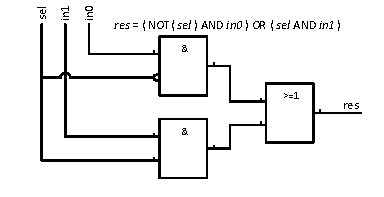
\includegraphics[scale=2]{./grafiken/ComparchUni_U1_A2_a.pdf}
\end{center} 

Unsere Implementierung eines Multiplexers nutzt ein Signal \texttt{temp1}, das temporär den Ausgabewert speichert, bevor dieser unverändert an \texttt{res} ausgegeben wird.
So vermeiden wir einen undefinierten Ausgabewert, da \texttt{temp1} mit dem Wert \texttt{0} initialisiert wird. 
Ansonsten könnte statt der Zwischenspeicherung in \texttt{temp1} auch eine direkte Ausgabe an \texttt{res} erfolgen.

\lstinputlisting[]{../multiplexer/multiplexer.vhd}


\textbf{Testbench: 2-Eingaben-Multiplexer (multiplexer\_tb.vhd)}

In unserer Testbench definieren wir zunächst die Ports und benötigten Signale. Wir verwenden keinen Clock, da es sich um eine asynchrone Schaltung handelt.

\lstinputlisting[linerange=1-24, firstnumber =1]{../multiplexer/multiplexer_tb.vhd}

Wir erstellen ein Array, das alle möglichen In- und Outputkombinationen des Multiplexers enthält, entsprechend eine Wahrheitstabelle.

Diese werden in unserer Testschleife verwendet, um nacheinander alle Szenarien abzuarbeiten und das tatsächliche Ergebnis mit dem erwarteten Ergebnis in einer assert-Abfrage abzugleichen.

Mit zahlenreichen Konsolenausgaben kann der Test einfach verfolgt und ein potentieller Fehler schnell entdeckt werden.

\lstinputlisting[linerange=26-82, firstnumber =26]{../multiplexer/multiplexer_tb.vhd}



\subsection{1-Bit-Multiplizierer (einBitMulti.vhd)}

Der 1-Bit-Multiplizierer entspricht einem \texttt{AND}-Gate, da kein Carry-Bit erwartet wird. Dementsprechend einfach ist der eigentliche Schaltkreis.

Wie in der ersten Aufgabe nutzen wir ein temporäres und mit 0 initiiertes Signal, um keine Ungewissheit über initiale Signalwerte zu haben.

\begin{align*}
res &= in0 \wedge in1
\end{align*}

\begin{center}
	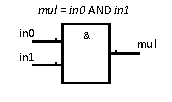
\includegraphics[scale=2]{./grafiken/ComparchUni_U1_A2_b.pdf}
\end{center} 

\lstinputlisting[]{../einBitMulti/einBitMulti.vhd}

\textbf{Testbench: 1-Bit-Multiplizierer (einBitMulti\_tb.vhd)}

Auch in diesem Testbench verzichten wir auf einen Clock und überprüfen die Korrektheit der Entität mit einer
Wahrheitstabelle. Diese fällt aufgrund der Einfachheit der Entität bedeutend einfacher aus.

\lstinputlisting{../einBitMulti/einBitMulti_tb.vhd}


\subsection{4-Bit-Multiplizierer}

Der 4-Bit-Multiplizierer gestaltet sich etwas komplexer in der Lösung als die vorherigen Aufgaben:

Unser Lösungsansatz ist, den Multiplikator mit den einzelnen Stellen (Bits) des Faktors zu multiplizieren (von rechts nach links). So erhalten wir immer den ursprünglichen Wert des Multiplikators oder 0 als Ergebnis.

Nach jeder Multiplikation die nächste Multiplikation um ein Bit nach links zu verschieben, sodass immer größere Zahlen entstehen. Anschließend werden alle Zwischenergebnisse in einem 8-Bit-Addierer zusammengerechnet und wir erhalten den multiplizierten Wert.

\begin{center}
	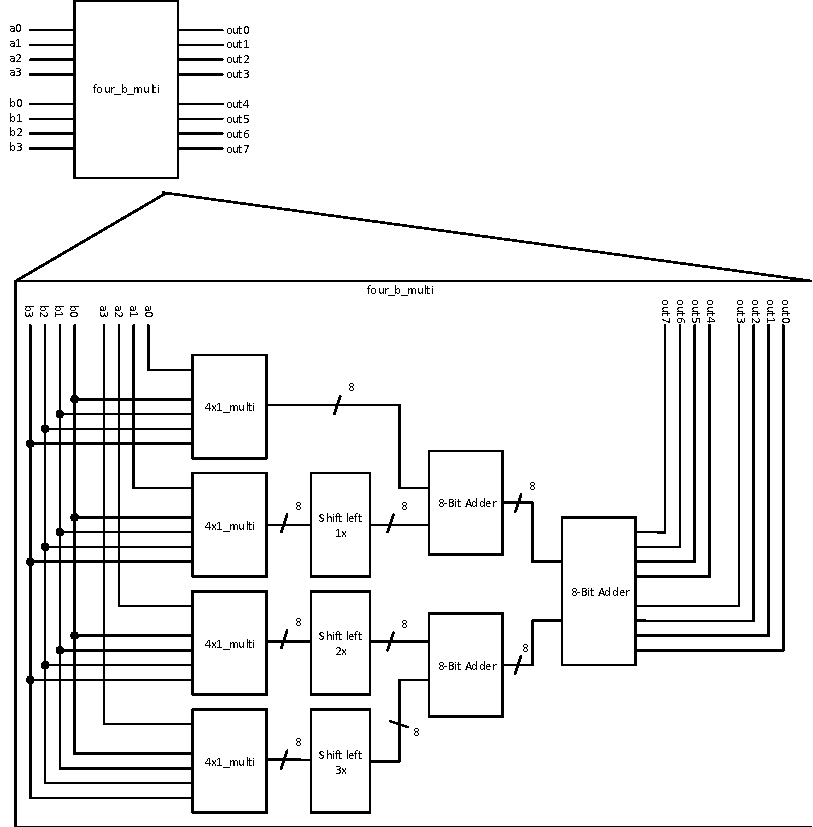
\includegraphics[scale=1.2]{./grafiken/ComparchUni_U1_A2_c.pdf}
\end{center} 

\newpage
In dem folgenden Beispiel wird der prinzipielle Ablauf unserer Multiplikationsberechnung beschrieben:
\begin{align*}
\text{Faktor}&=1011\\
\text{Multiplikator}&=1101\\
\\
\text{1. Stelle d. Faktors} \cdot \text{Multiplikator}&= 1 \cdot 1101\\
&=1101\\
\\
\text{2. Stelle d. Faktors} \cdot \text{Multiplikator}&= 1 \cdot 1101\\
&=1101\\
\text{[...] mit Bitshift}&= 11010\\
\\
\text{3. Stelle d. Faktors} \cdot \text{Multiplikator}&= 0 \cdot 1101\\
&=0\\
\text{[...] mit Bitshift}&= 0\\
\\
\text{4. Stelle d. Faktors} \cdot \text{Multiplikator}&= 1 \cdot 1101\\
&=1101\\
\text{[...] mit Bitshift}&= 1101000\\
\begin{aligned}[t]
1011 &\\
\times  1101& \\
\hline
1101&\\
+11010&\\
+000000&\\
+1101000&\\
\hline
{\scriptscriptstyle1} \; \; \; \; \; \; \; \,\\
+1111111\\
\hline
10001111
\end{aligned}
\end{align*}

Die Zwischenergebnisse dieser Rechnung werden jeweils in den Signalen \texttt{tmp0} bis \texttt{tmp6} gespeichert. 

Wir nutzen einen 8-Bit-Addierer, den wir in einer zusätzlichen Datei namens \texttt{eight\_bit\_adder.vhd} gespeichert haben, um die Zwischenergebnisse zu einem Gesamtergebnis zu addieren.

\lstinputlisting{../vierBitMulti/four_b_multi.vhd}

\subsection*{Für Aufgabe 2.3: Vier-Bit-Addierer (eight\_bit\_adder.vhd)}

Den Volladdierer und die Testbench des Volladdierers haben wir aus den auf StudIP hochgeladenen Dateien entnommen.

Der Acht-Bit-Addierer gestaltet sich als vergleichsweise unkompliziert. Wir führen die einzelnen Additionen mit acht Volladdierern aus, die das Carry-Bit (\texttt{tmp0} bis \texttt{tmp7}) des jeweils vorherigen Volladdierers nutzen, um die nächste Stelle des Ergebnisses zu berechnen. Jeder Volladdierer errechnet so das Ergebnis einer einzelnen Stelle.

Der Volladdierer ist in \texttt{full\_adder.vhd} näher beschrieben.

\lstinputlisting{../vierBitMulti/eight_bit_adder.vhd}

\subsection*{Für Aufgabe 2.3: Volladdierer (full\_adder.vhd)}
Der Volladdierer operiert auf folgende Weise:

\texttt{a} und \texttt{b} sind die zu addierenden Bits, \texttt{c\_in} ist das Input-Carry, \texttt{c\_out} das Output-Carry und \texttt{s} das Ergebnis der Addition.

\begin{align*}
s &= a \veebar b \veebar c\_in\\
c &= (a \vee b) \wedge (a \vee c\_in) \vee (b \wedge c\_in))
\end{align*}

\lstinputlisting{../vierBitMulti/full_adder.vhd}

\section{Geisterfigur (ghost.vhd)}

Wir nutzen zwei Eingänge, den Bewegungssensor \texttt{move} und den Clock \texttt{clk}, um das Ergebnis der Ausgänge zu bestimmen. 

\lstinputlisting[linerange=1-14, firstnumber =1]{../ghost/ghost.vhd}

Erneut nutzen wir Signale, damit die Werte zu Beginn der Simulation eindeutig sind. Dabei werden \texttt{speaker} für \texttt{chains} und \texttt{bulb} für \texttt{eyes} in jedem Clock-Cycle als Wert zugewiesen. 

\lstinputlisting[linerange=16-24, firstnumber =16]{../ghost/ghost.vhd}

Nachdem der Bewegungssensor überprüft wurde, werden abhängig davon, ob Bewegung festgestellt wurde, verschiedene Signale hochgezählt, um die Tätigkeiten der Figur in korrekter Zeit und Reihenfolge ablaufen zu lassen. In Zeile 35-47 wird der Code bei Bewegung beschrieben und in Zeile 49-63 wird beschrieben, was passiert, wenn keine Bewegung festgestellt wurde.

Es wird jeweils \texttt{counterON} bzw. \texttt{counterOFF} genutzt, um den zeitlichen Ablauf zu definieren. So wird beispielsweise \texttt{bulb} auf 0 gesetzt, wenn \texttt{counterOff} 30 erreicht.

\lstinputlisting[linerange=26-71, firstnumber =26]{../ghost/ghost.vhd}

\texttt{speaker} und \texttt{bulb} müssen natürlich ihren Wert an die Outputs übergeben, die sie stellvertreten.

\lstinputlisting[linerange=73-79, firstnumber = 73]{../ghost/ghost.vhd}

\subsection*{Testbench: ghost\_tb.vhd}

Unsere Testbench überprüft, ob \texttt{ghost} beim üblichen Betriebsablauf die Outputs korrekt setzt. 
		
Indem vor und nach dem Auslösen des Bewegungsmelders zu verschiedenen Zeitpunkten mir einer Assert-Abfrage überprüft wird, ob die Outputs zu genau diesem Clock-Cycle wie erwartet sind, können wir den gesamten Ablauf überprüfen. 

Der erste und letzte Schritt unseres Tests überprüft, ob die Outputs 0 ausgeben. So können wir ein unerwartetes oder verspätetes Verhalten der Figur ausschließen.

Mit zahlreichen \texttt{report}-Befehlen bleibt der Tests gut verfolgbar, um mögliche Fehlerquellen zu entdecken.

\lstinputlisting{../ghost/ghost_tb.vhd}
\end{document}